\documentclass{beamer}
\usepackage{scrextend}
\usepackage{amsfonts}
%\usepackage[T1]{fontenc}
\usepackage{booktabs}
\usepackage[latin1]{inputenc}
\usepackage{graphicx}
\usepackage{mathtools}
\usepackage{multimedia}
\usepackage{url}
\usepackage{tikz}
\setbeamertemplate{caption}{\raggedright\insertcaption\par}
\usepackage{pstricks,pst-node}
%Packages Tableaux
\usepackage{tabularx} %Tableaux
\usepackage{multirow} %Gestion des lignes
\usepackage{multicol} %Gestion des colones
\usepackage{fancybox} %Boites
\usepackage{multicol} %Colonnes
\usepackage{array} %Tableaux maths
\usepackage{fancybox}
\usetikzlibrary{arrows} 
\usepackage[linesnumbered,titlenotnumbered,ruled,vlined]{algorithm2e}
\renewcommand{\thealgocf}{}
\usetheme{Ilmenau}
\addtobeamertemplate{footline}{\hfill\hspace*{-0.1cm}\insertframenumber/\inserttotalframenumber\hspace{2em}\null}

\title[Master of Science in Informatics at Grenoble: Master Thesis Defence]{Inverse Procedural Generation of Geological Stories}
\author{Garcia Maxime}
\institute{Mosig GVR}
\date{June $23^{th}$ 2016}


\begin{document}

	
    \begin{frame}[label=(intro)]
	\titlepage
    \end{frame}
	
	 \begin{frame}
	 \frametitle{Our Context}
	 \begin{itemize}
	 \item Retrieve terrains's history
	 \item Date geological events. Better understand terrain formation
	 \item Analyse geological sketches 
	 \item Identify areas where oil and other ressources are trapped
	 \end{itemize}
	 	\begin{figure}[H]
	\centering
	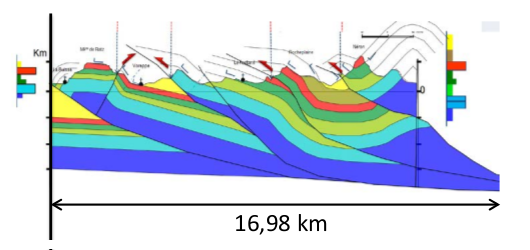
\includegraphics[scale=0.5]{Wraped_Section.png}
		\end{figure}
	 \end{frame}
	
	\begin{frame}
	\frametitle{Introduction}
	\begin{itemize}
	\setbeamertemplate{itemize item}[ball]
	\item Cross Section Restoration process
	\setbeamertemplate{itemize item}[ball]
	\item Retrieve the history of a cross section (Geological Events)
	\item Different kind of events to un-do:\\ 
	\begin{itemize}
		\item sedimentation, erosion, foldings, faulting
	\end{itemize}
	\begin{figure}[H]
	\centering
	\hspace*{-0.3cm}
	\begin{tabular}{@{}cc@{}}
	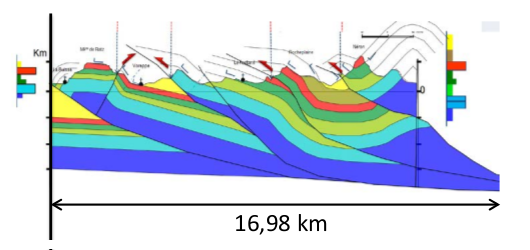
\includegraphics[width=.49\textwidth]{Wraped_Section.png}&
	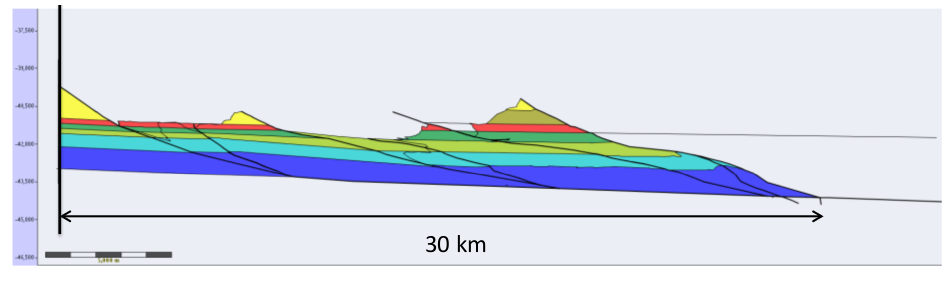
\includegraphics[width=.48\textwidth]{UnWraped_Section.png}\\
	\end{tabular}
	\end{figure}
	\end{itemize}
	\end{frame}

	\begin{frame}
	\frametitle{Our contributions}
	\begin{itemize}
	\item Event Graph generation, detect and rank events (automatic)
	\item Backward simulation using mass-spring systems (automatic)
	\item Story graph generation, create and simulate restoration scenarios (interactive)
	\end{itemize}
    \end{frame}	
	
	\begin{frame}
	\frametitle{State of the Art}
	\begin{itemize}
	\item Geological state of the art:
		\begin{itemize}
		\item Geometrically-based methods
		\item Physically-based methods
		\end{itemize}
	\item Graphics state of the art
		\begin{itemize}
		\item Sketch-based method
		\end{itemize}
	\end{itemize}
    \end{frame}

	 \begin{frame}
	\frametitle{Geometrically based restoration methods: 2D Move 
  
\includegraphics[scale=0.13]{Move_logo_-01.png}}
	 \begin{figure}[H]
	\centering
	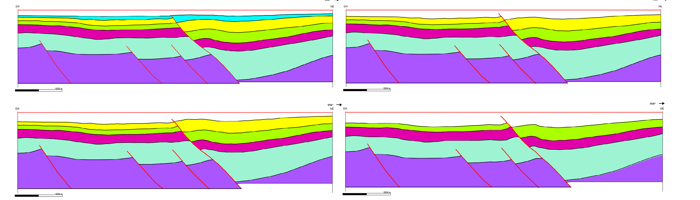
\includegraphics[scale=1.8]{mve2Dmini.png}
	\label{mve}
	\end{figure}
	\begin{columns}
	\begin{column}{0.55\textwidth}
	\begin{itemize}
	\item Interactive methods: flatten layers, move blocks, remove or add matter
	\item Kinematic algorithms $\longrightarrow$ preserve geometrical and geological coherence
	\end{itemize}
	\end{column}
	\begin{column}{0.55\textwidth}
	\begin{itemize}
	\item Take into account many geological events (erosion, sedimentation, foldings, faults, compaction)
	\end{itemize}
	\end{column}
	\end{columns}
    \end{frame}   
    
     \begin{frame}
	\frametitle{Geometrically based restoration methods: 3D Move 
  
\includegraphics[scale=0.13]{Move_logo_-01.png}}
	 \begin{itemize}
	 \item 3D aspect of terrains using a 3D model and several cross sections:
	 \end{itemize}
	 \begin{figure}[H]
	\centering
	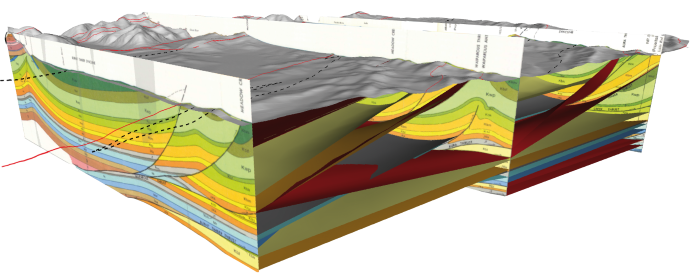
\includegraphics[scale=1.7]{mve3D.png}
	\label{mve3}
	\end{figure}
		\footnotetext{\url{http://www.mve.com/software/move}}
    \end{frame}   
    
	\begin{frame}
	\frametitle{Physically-based methods}
	\begin{itemize}
	\item Run mecanical simulation over an input section
	\item Use finite elements methods with Coulomb theory
	\item Two kinds: Forward and Backward simulations
	\end{itemize}
    \end{frame}    
    
    \begin{frame}
	\frametitle{Forward physic simulations}
	\begin{itemize}
	\item Run the simulation over the restoration
	\item Simulate many kinds of geological events
	\item Compare the final result with the Cross Section current state $\longrightarrow$ Validate the restoration process
	\end{itemize}
	
	\begin{figure}[H]
	\centering
	\href{slamtec.mp4}{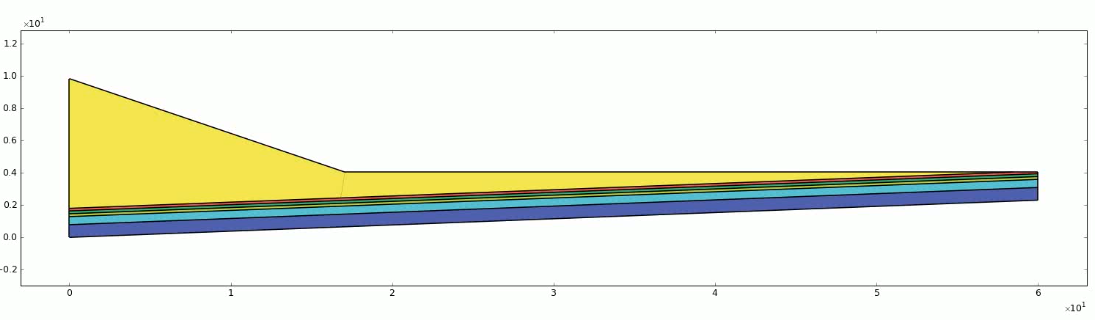
\includegraphics[scale=0.25]{slamim.png}}
	\end{figure}
	\footnotetext{\url{https://www.u-cergy.fr/fr/laboratoires/laboratoire-gec/equipement/logiciels.html}}
    \end{frame}
    
    
    \begin{frame}
	\frametitle{Backward physic simulations: Dynel 2D \fbox{
\includegraphics[scale=0.5]{dyn2Dlogo.png}}}
	\begin{columns}
	\begin{column}{0.55\textwidth}
	\begin{figure}[H]
	\centering
	\vspace*{-0.5cm}
	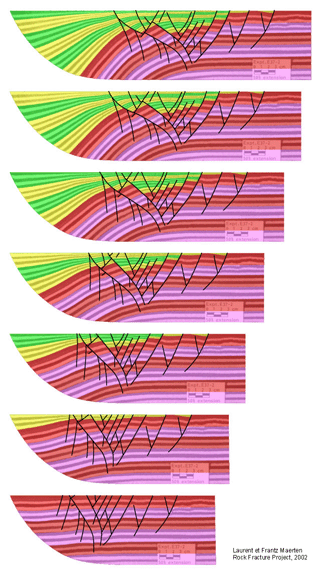
\includegraphics[scale=0.3]{dynel2D.png}
	\label{dyn2}
	\end{figure}
	\end{column}
	\begin{column}{0.55\textwidth}
	\begin{itemize}
	\item Run the simulation over the Cross Section current state
	\item Inverse the way event were applied. Run a forward simulation of these inverted events
	\item Many uncertainties on identifying events to "un-do"
	\end{itemize} 
	\end{column}
	\end{columns}
	\footnotetext{\url{http://www.software.slb.com/-/media/software/documents/external/product\%20sheets/dynel_2d_ps.pdf}}
    \end{frame}
    	
	\begin{frame}
	\frametitle{Sketch Based method}
	 \begin{figure}[H]
	\centering
	\vspace*{-0.5cm}
	\begin{tabular}{@{}cc@{}}
	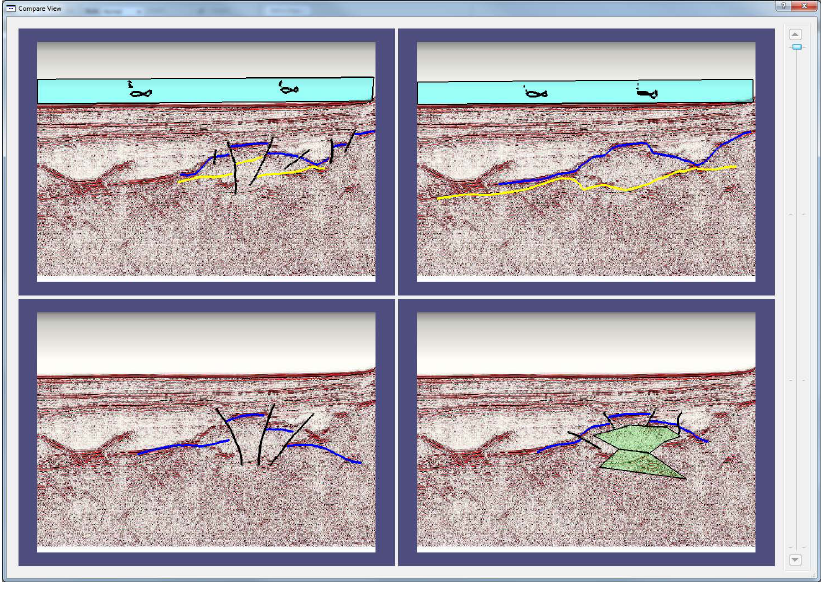
\includegraphics[width=.42\textwidth]{lidal0.png}&
	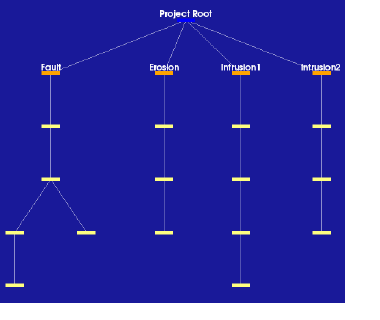
\includegraphics[width=.42\textwidth]{lidal1.png}\\
	\end{tabular}
	\label{lidal}
	\end{figure}
	\begin{columns}
	\begin{column}{0.60\textwidth}
	\vspace*{-0.5cm}
	\begin{itemize}
	\item More recent methods.\\ Few works done on it
	\item Traditionnal way of restoring by drawing
	\end{itemize}
	\end{column}
	\begin{column}{0.60\textwidth}
	\begin{itemize}
	\item Organize drawings in a story tree 
	\item Draw by superimposing them
	\end{itemize}
	\end{column}
	\end{columns}
	\footnotetext{Lidal and al. Geological storytelling. Computers \& graphics}
	\end{frame} 
	
	\begin{frame}
	\frametitle{State of the art: limitation and new challenges}
	\begin{itemize}
	\item Geological methods: 
		\begin{itemize}
		 \item Only one scenario proposed when restoring
		 \item Geologists spend too much time adjusting initial conditions
		 \item Geometrically-based methods don't provide inbetween animation
		\end{itemize}
	\item Graphics methods:
	\begin{itemize}
	\item Not automatic method (no events porposed)
	\item No animation $\longrightarrow$ no coherence guatantee
	\item Takes time to draw multiple scenarios
	\end{itemize}
	\end{itemize}
    \end{frame}	
    
    \begin{frame}
	\frametitle{Our method: general principle}
	 \begin{figure}[H]
	\centering
	\includegraphics[scale=0.40]{mainGoal2.png}
	\label{maingoal}
	\end{figure}
	\end{frame}
       
	\begin{frame}
	\frametitle{Our method: processing pipeline}
	\begin{columns}
	\begin{column}{0.58\textwidth}
	  \scalebox{0.85}{
	  \hspace*{0.1cm}
	\begin{algorithm}[H]
	 \KwData{Input cross section}
	 \KwResult{Cross section history forward animation }
	 Extract geological and topological data from the input (automatic)\;
	 Map mass-spring system on the cross section (automatic)\;
	 Detect and rank events to un-do: Event Graph Generation (automatic)\;
	 \eIf{chooseEvent(t,storyTree)}{generateForwardAnimation(storyTree)}{\Return\;}

	 \caption{Restoration process}
	\end{algorithm}
	}
	\end{column}
	\begin{column}{0.62\textwidth}
	\scalebox{0.72}{
	\begin{algorithm}[H]
	\DontPrintSemicolon 
	\KwIn{$t$ a time step, storyTree the story tree the user is building}
	\KwOut{restoration success boolean}
	System generate a list of possible event to un-do\;
	\If{possibleEventList is empty}{\Return true \;}
	\eIf{user choose events in the list}{addNode(storyTree,t,possibleEventList)\;addEdge(storyTree,t,choosenEvents)\;
	SimulateBackward(choosenEvents)\;
	\eIf{chooseEvent($t + 1$, storyTree)}{\Return true\;}{\Return chooseEvent($t$, storyTree)\;}}
	{\Return false\;}
	\caption{chooseEvent}
	\end{algorithm}
	}
	\end{column}
	\end{columns}
	\end{frame}
	
	\begin{frame}
	\frametitle{General Pipeline}
	 \begin{figure}[H]
	\centering
	\includegraphics[width=\textwidth, height=0.8\textheight]{generalPipeline.png}
	\label{maingoal}
	\end{figure}
	\end{frame}	
	

	
	\begin{frame}
	\frametitle{Geological Events List}
	\begin{columns}
	\begin{column}{0.55\textwidth}
	\begin{figure}[H]
	\centering
	\begin{tabular}{@{}ccc@{}}
	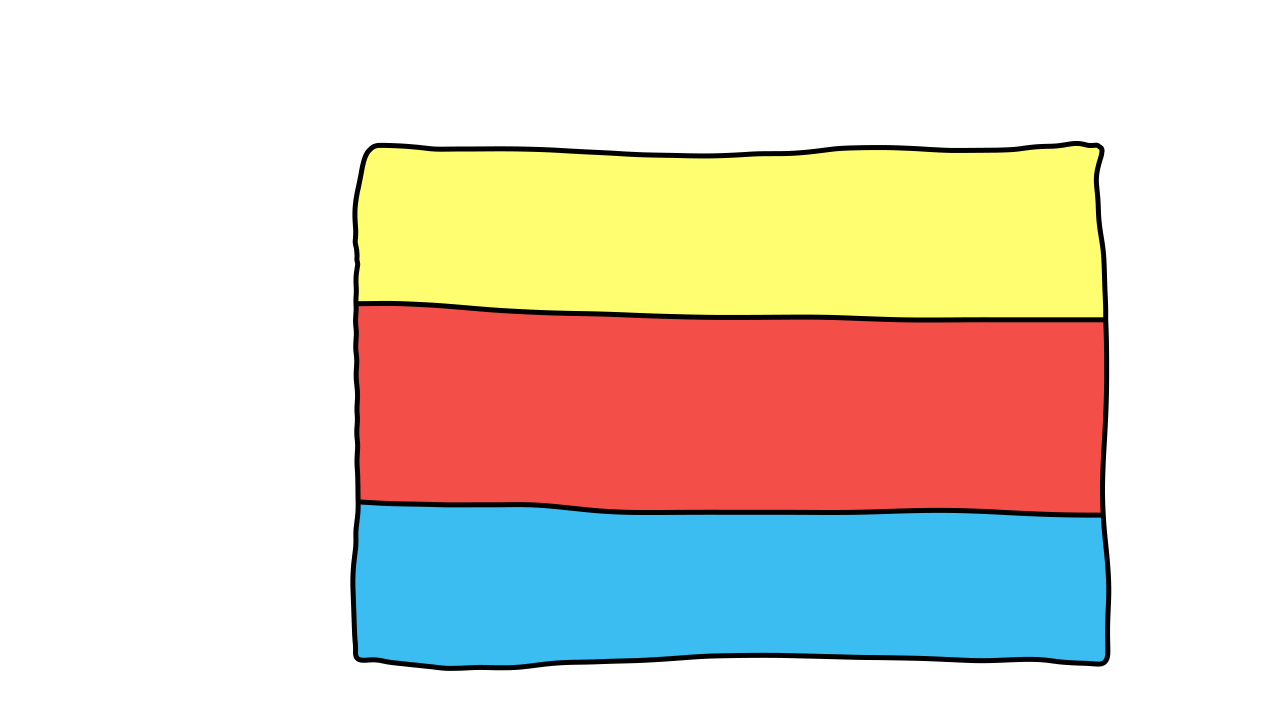
\includegraphics[width=.34\textwidth]{unSedimentDescription0.png}&
	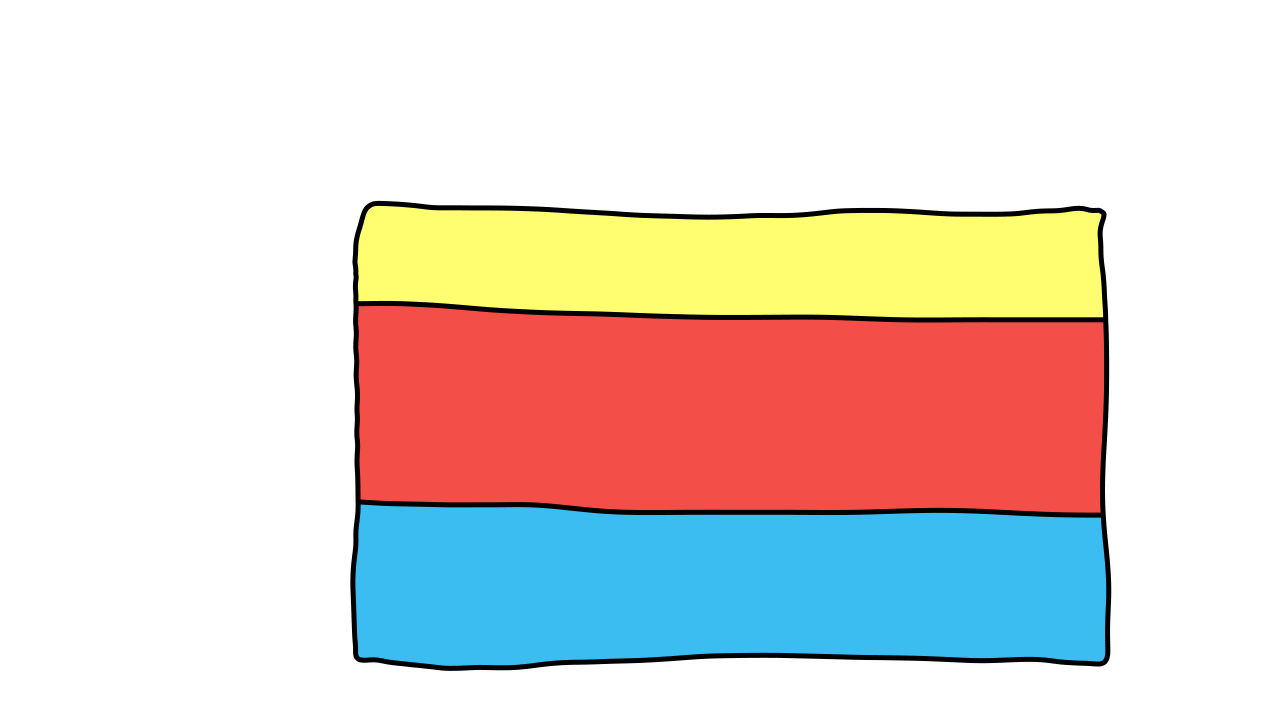
\includegraphics[width=.34\textwidth]{unSedimentDescription1.png}&
	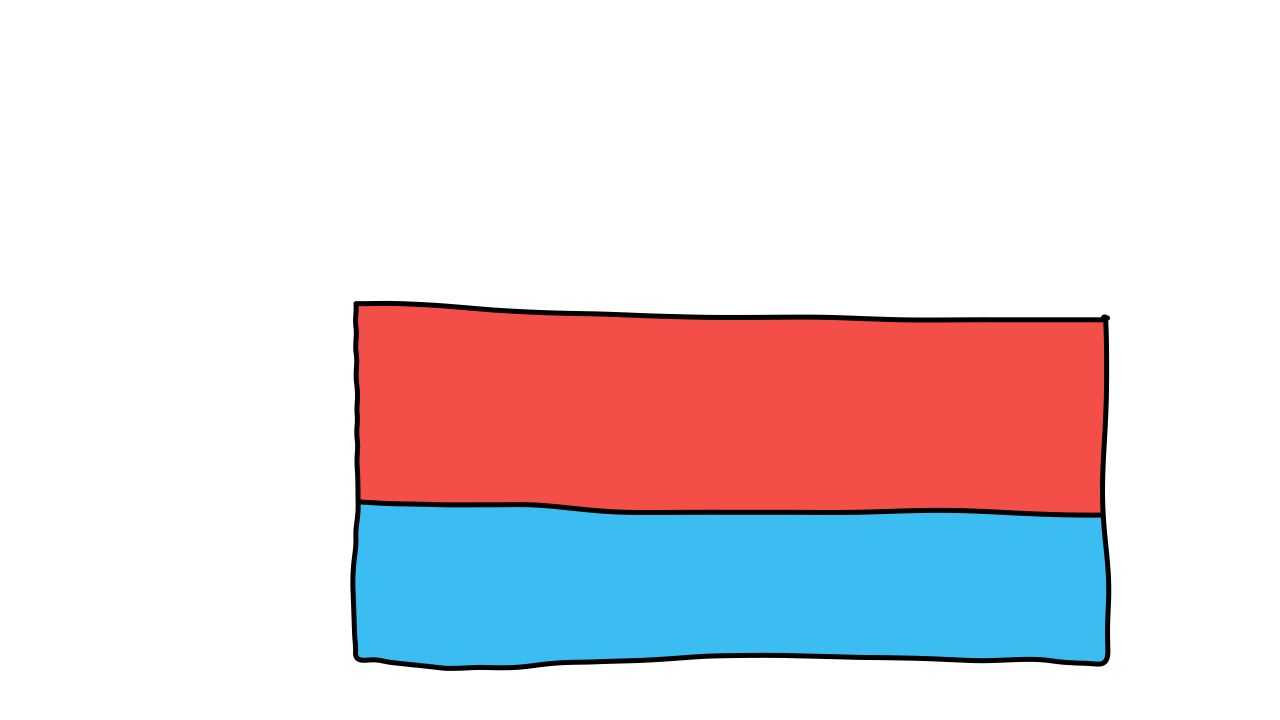
\includegraphics[width=.34\textwidth]{unSedimentDescription2.png}\\
	\end{tabular}
	\caption{Un-Sediment}
	\label{unsedeg2}
	\end{figure}
	\begin{figure}[H]
	\centering
	\begin{tabular}{@{}ccc@{}}
	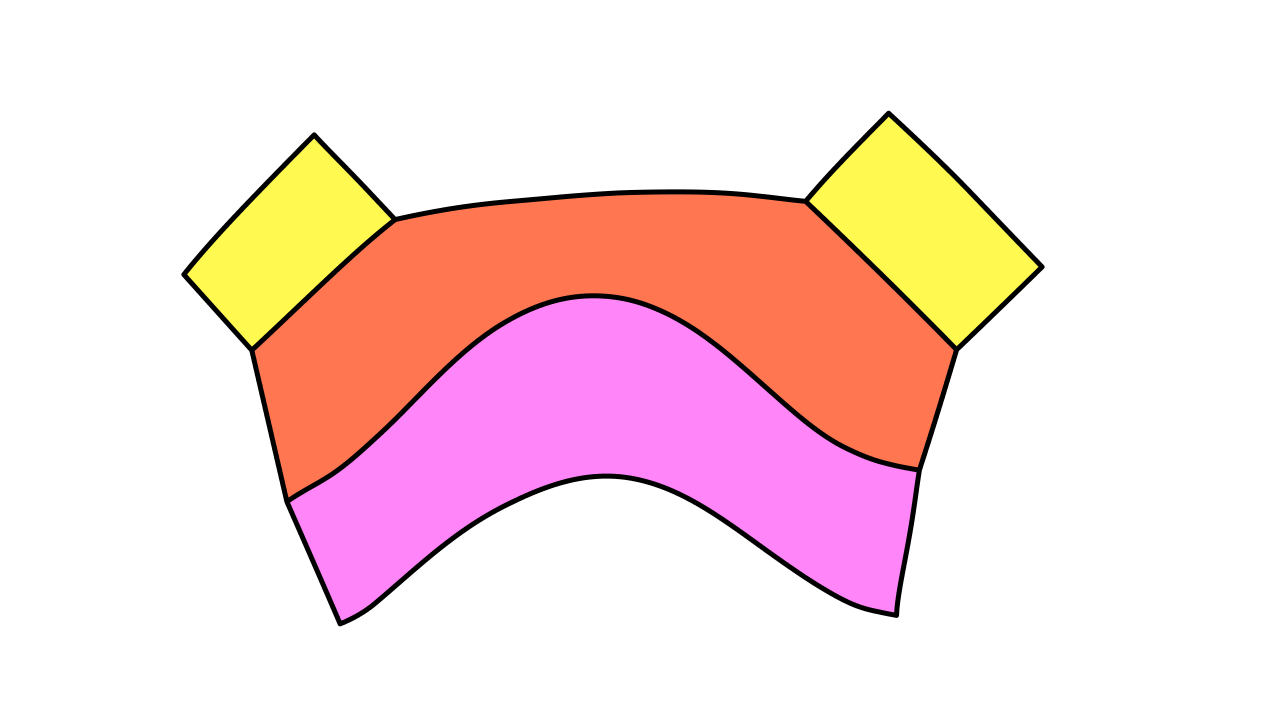
\includegraphics[width=.34\textwidth]	{unErodeConvexDescription0.png}&
	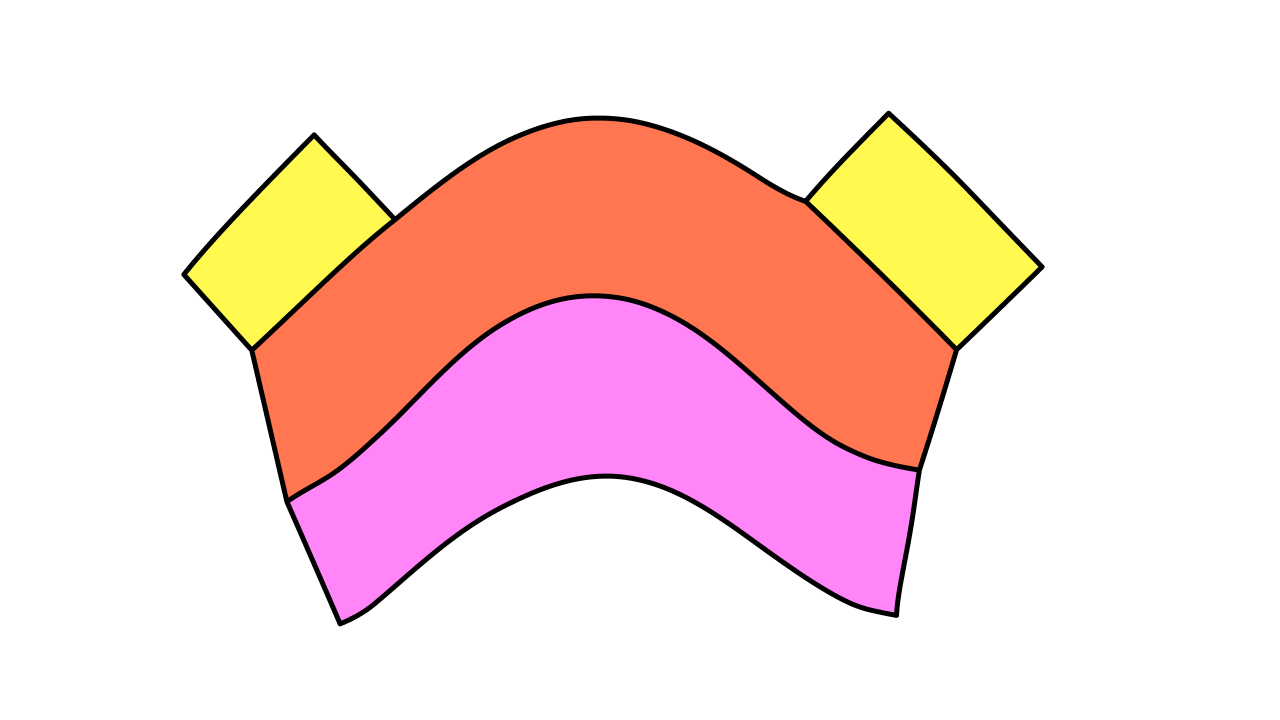
\includegraphics[width=.34\textwidth]{unErodeConvexDescription1.png}&
	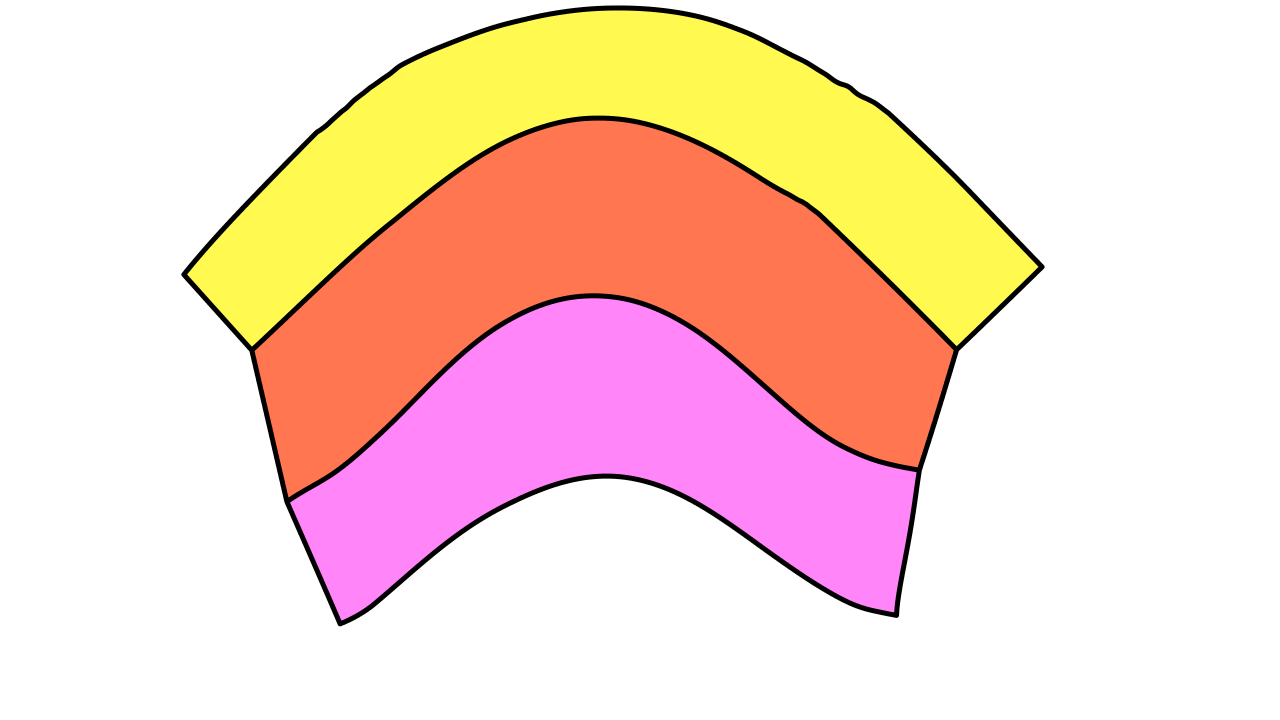
\includegraphics[width=.34\textwidth]	{unErodeConvexDescription2.png}\\
	\end{tabular}
	\caption{Un-Erode}
	\label{unerodecveg}
	\end{figure}
	\end{column}
	\begin{column}{0.55\textwidth}
	\begin{figure}[H]
	\centering
	\begin{tabular}{@{}cc@{}}
	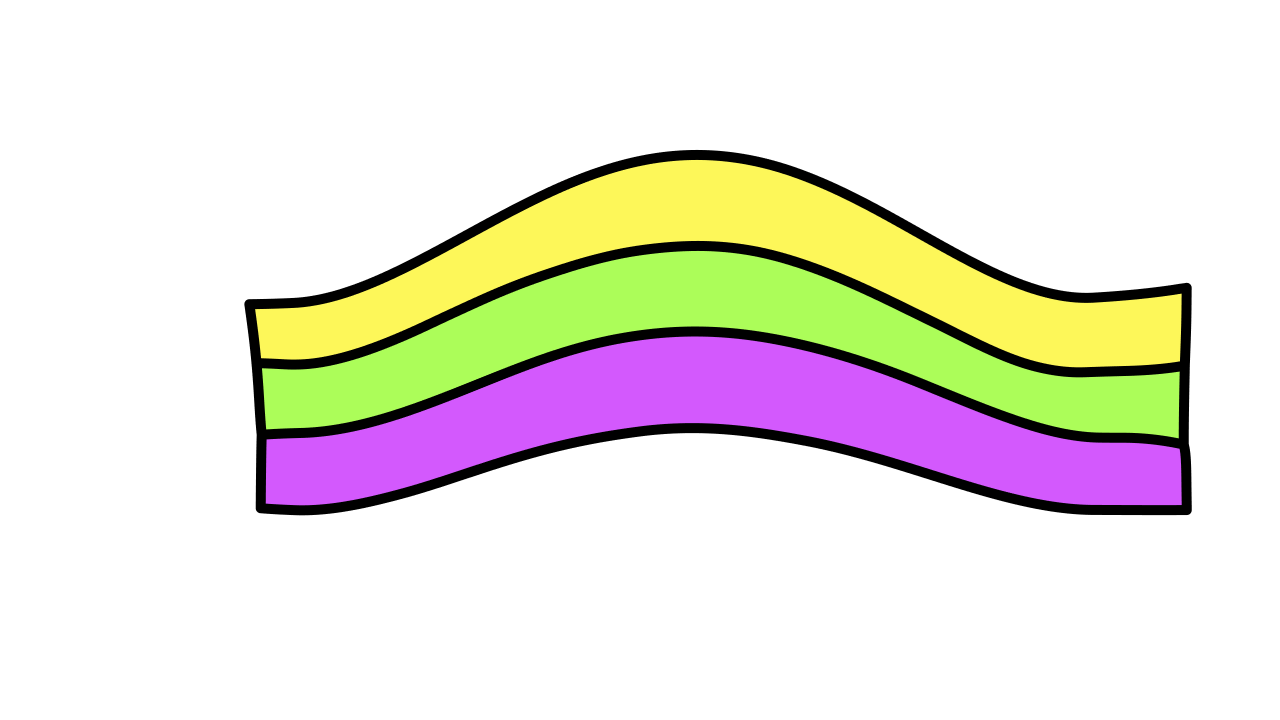
\includegraphics[width=.35\textwidth]{unFoldDescription0.png}&
	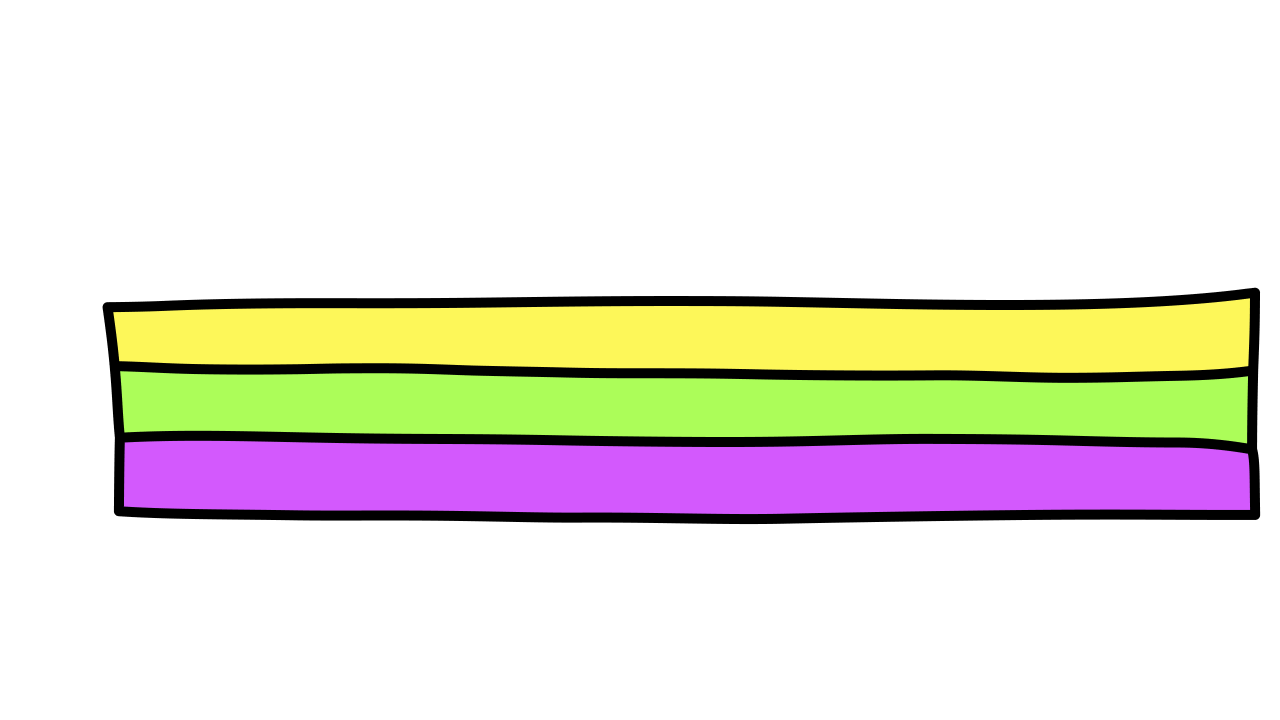
\includegraphics[width=.35\textwidth]{unFoldDescription1.png}\\
	\end{tabular}
	\caption{Un-Fold.}
	\label{unfoldeg}
	\end{figure}
	\begin{figure}[H]
	\centering
	\begin{tabular}{@{}cc@{}}
	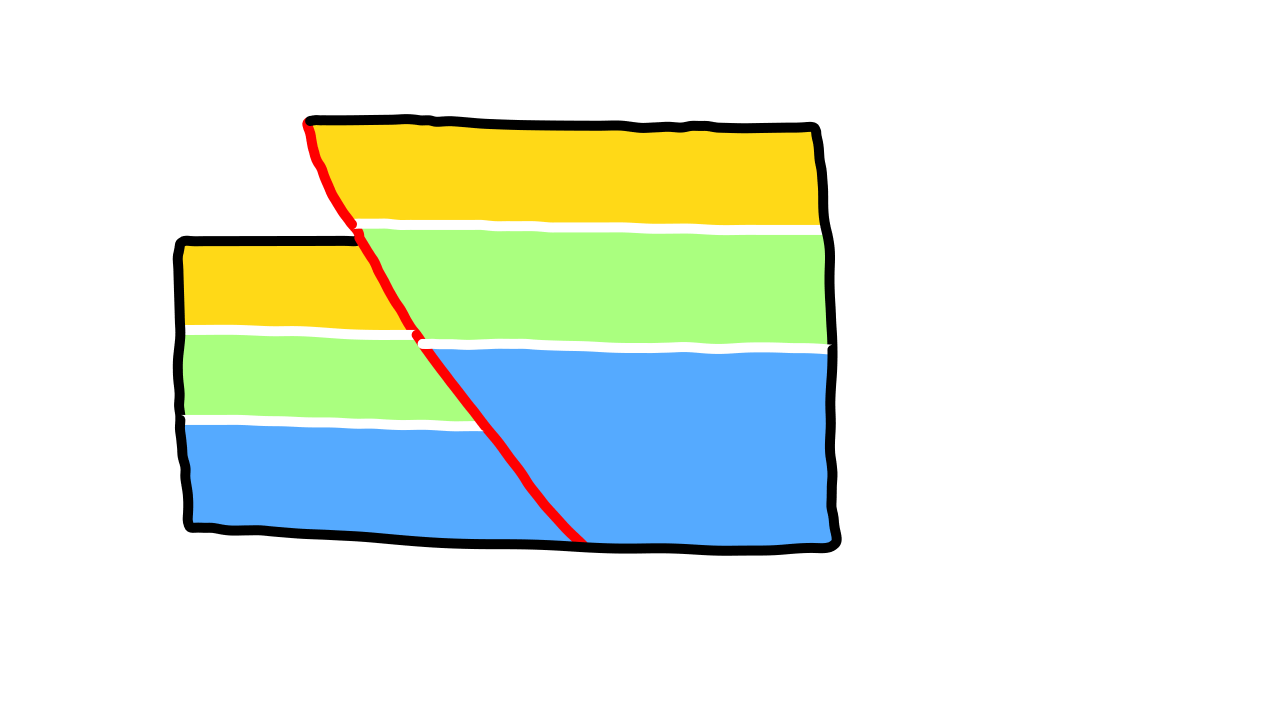
\includegraphics[width=.35\textwidth]{unFaultDescription0.png}&
	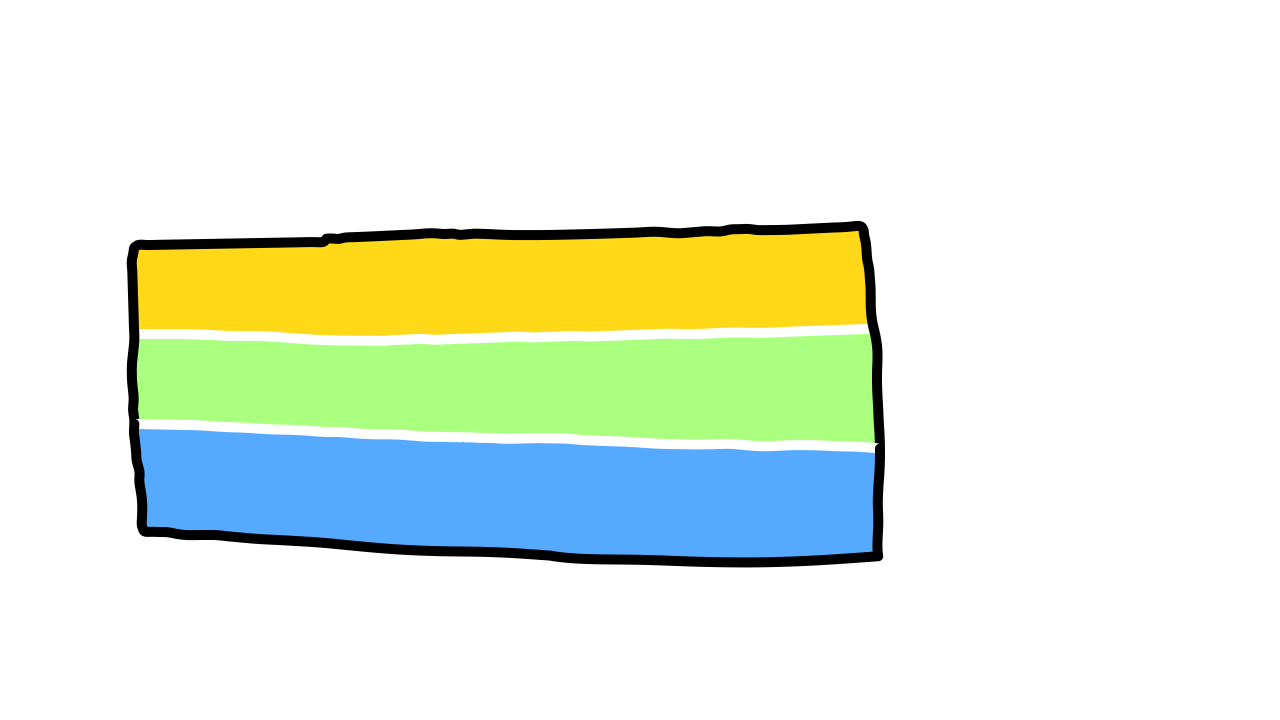
\includegraphics[width=.35\textwidth]{unFaultDescription1.png}\\
	\end{tabular}
	\caption{Un-Fault}
	\label{unfaulteg}
	\end{figure}
	\end{column}
	\end{columns}
	\end{frame}	
		
	\begin{frame}
	\frametitle{Event Graph generation : sketch analysis}
	\begin{figure}[H]
	\centering
	\vspace*{-1cm}
	\begin{tabular}{@{}cc@{}}
	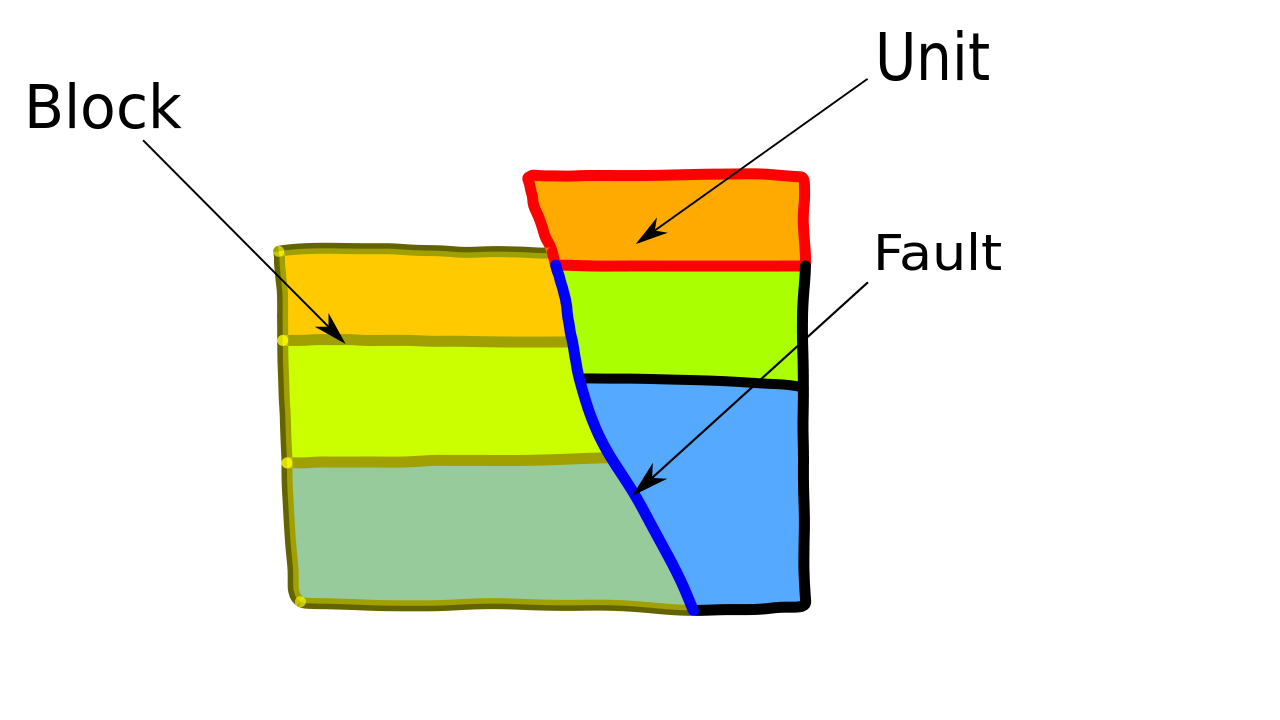
\includegraphics[width=.49\textwidth]{geologyStructEdit.png}&
	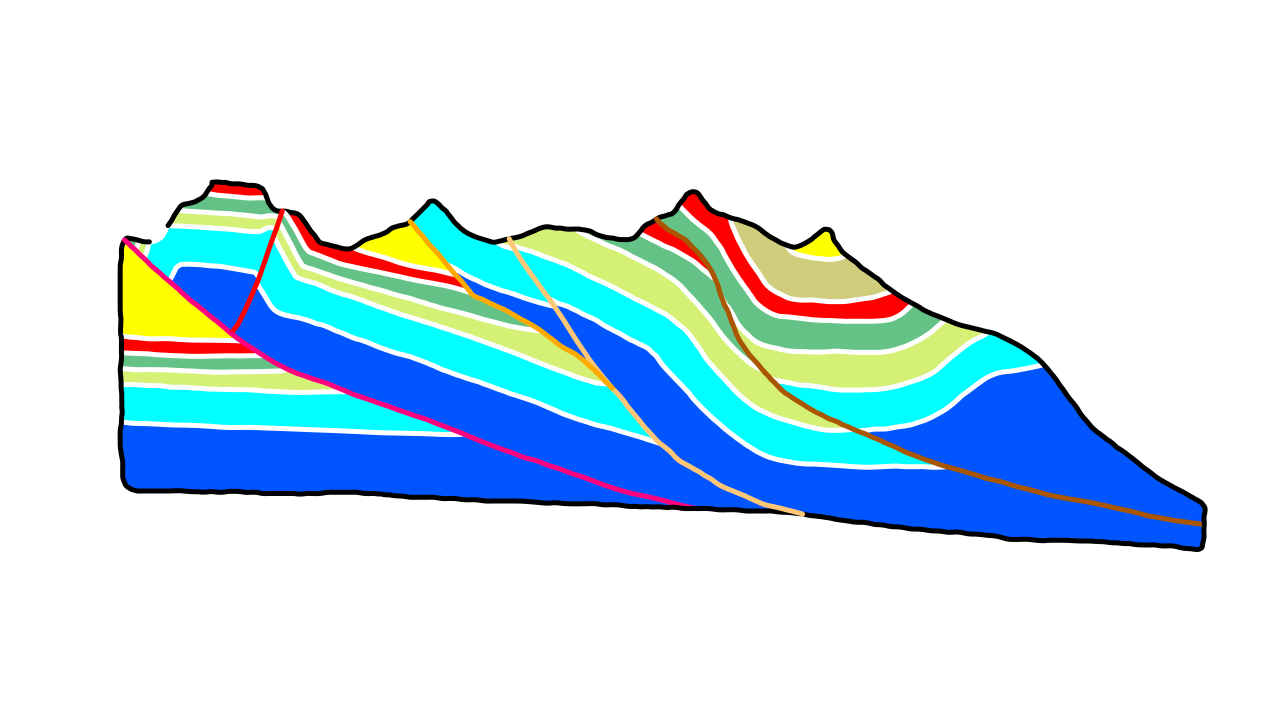
\includegraphics[width=.58\textwidth]{chartreusevpaint.png}\\
	\end{tabular}
	\label{unfaulteg}
	\end{figure}
	\vspace*{-1cm}
	\begin{itemize}
	\item Vector Graphics Complex (VGC) as input
	\item Geological Structure extraction
	\item Event detection using topological and geological data.
	\item Organize, schedule events in a graph structure: Event Graph
	\end{itemize}
	\footnotetext{Boris Dalstein and al. Vector graphics complexes. ACM transactions on Graphics, Proceedings of ACM SIGGRAPH}
	\end{frame}			
	
	\begin{frame}
	\frametitle{Event Graph: Scheduling and Ranking events}
	\begin{itemize}
	\item Store all events that are identifiable at the input Cross section state
	\item Create time dependences bewteen them (first ranking)
	\item Add probability of occurence for each event $\longrightarrow$ computed with evalutation functions (second ranking)
	\item Evaluation functions depend on each event they are applied on (eg: fault and erosion).
	\end{itemize}
	\end{frame}
	
	\begin{frame}
	\frametitle{Event Graph representation}
	\begin{columns}
	\begin{column}{0.55\textwidth}
	\begin{figure}[H]
	\centering
	\begin{tabular}{@{}cc@{}}
	\vspace*{2cm}
	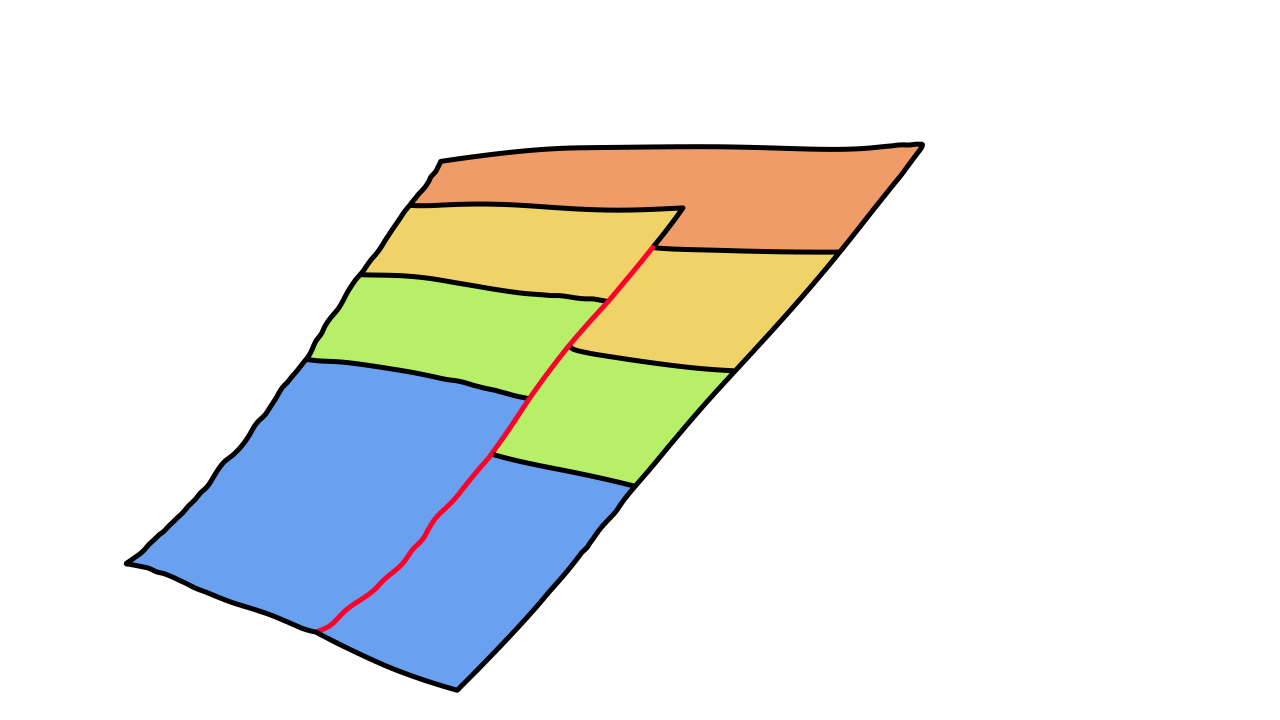
\includegraphics[width=.73\textwidth]{unFaultSedDescription.png}
	\includegraphics[width=.31\textwidth]{eventGraph.png}\\
	\end{tabular}
	\end{figure}
	\end{column}
	\begin{column}{0.55\textwidth}
	\begin{itemize}
	\item Oriented edges represent a time dependency between the pointed event and the pointing one
	\item The pointed event occured after the pointing one
	\item We will first un-do events with no incomming edges
	\end{itemize}
	\end{column}
	\end{columns}
	\end{frame}
			
	\begin{frame}
	\frametitle{Backward simulation: Mass-Spring systems}
	\begin{columns}
	\begin{column}{0.55\textwidth}
	\begin{itemize}
	\item Often used for simulating deformable objects (cloth)
	\item Implemented implicit euler scheme (more stable)
	\item Mapping along the level boundaries's gradient
	\end{itemize}
	\end{column}
	\begin{column}{0.55\textwidth}
	\begin{figure}[H]
	\centering
	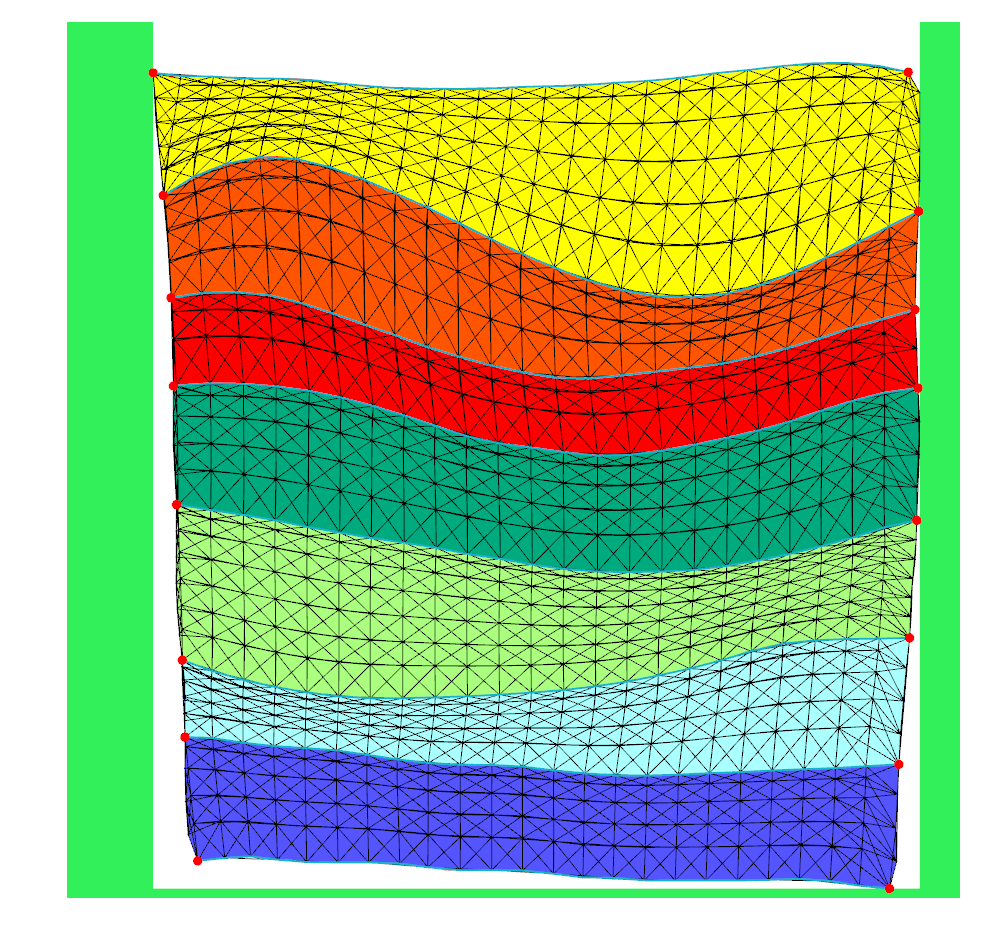
\includegraphics[scale=0.15]{springMapping.png}
	\end{figure}
	\end{column}
	\end{columns}
	\end{frame}
	
	\begin{frame}
	\frametitle{Implicit Euler Scheme}
	
	\begin{align}
	(v^{n+1} - v^n) &= (I - \frac{dt^2}{m}H)^{-1}(F^n + dt H v^n)\frac{dt}{m}
	\end{align}
	
	\begin{equation}
\textsl{Additionnal force: } F_{ij}^{torsion} = -k_{torsion}\Delta \theta \vec{n}
	\end{equation}
	
	\begin{figure}[H]
	\centering
	\begin{tabular}{@{}cc@{}}
	\includegraphics[width=.45\textwidth]{torsionForces.png}&
	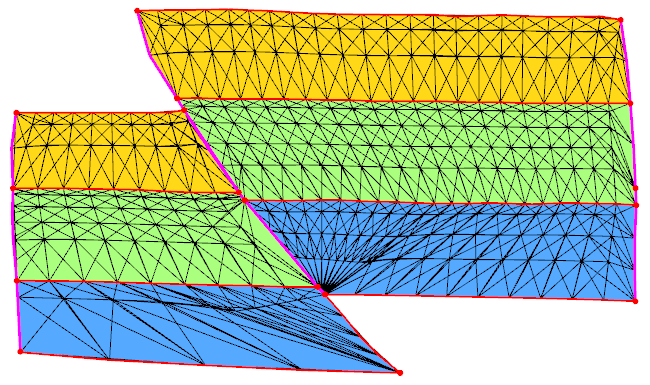
\includegraphics[width=.45\textwidth]{collisions.png}\\
	\end{tabular}
	\caption{Torsion and Collision}
	\end{figure}

	\end{frame}
	
	\begin{frame}
	\frametitle{Event Simulation: Geological operators}
	\begin{columns}
	\begin{column}{0.55\textwidth}
	\begin{figure}[H]
	\centering
	\begin{tabular}{@{}ccc@{}}
	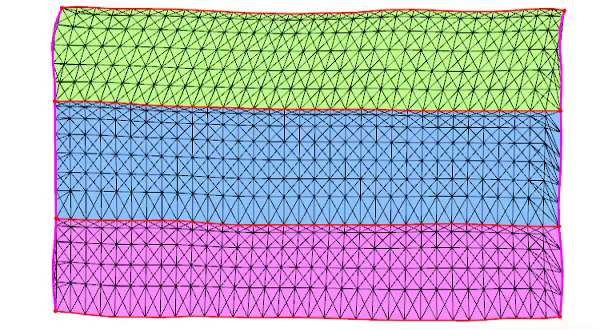
\includegraphics[width=.41\textwidth]{unSedimentMesh0.png}&
	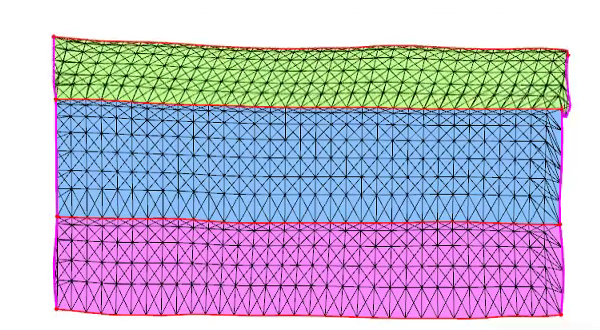
\includegraphics[width=.41\textwidth]{unSedimentMesh1.png}&
	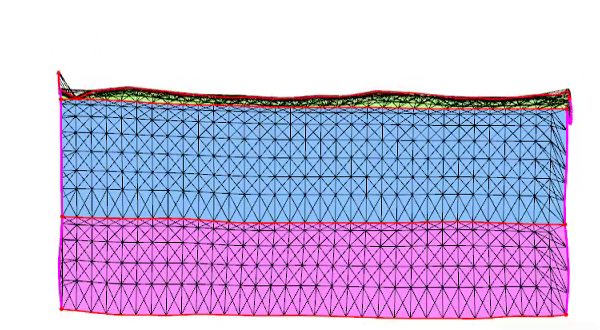
\includegraphics[width=.41\textwidth]{unSedimentMesh2.png}\\
	\end{tabular}
	\caption{Un-Sediment}
	\label{unsedeg2}
	\end{figure}
	\begin{figure}[H]
	\centering
	\begin{tabular}{@{}ccc@{}}
	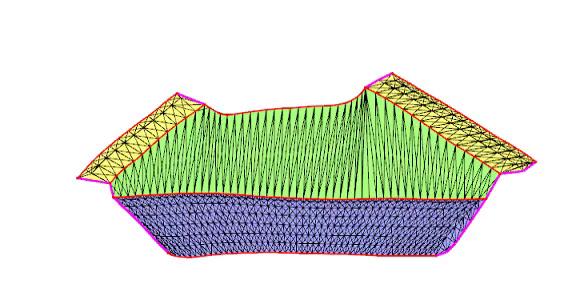
\includegraphics[width=.43\textwidth]{unErodeMesh0.png}&
	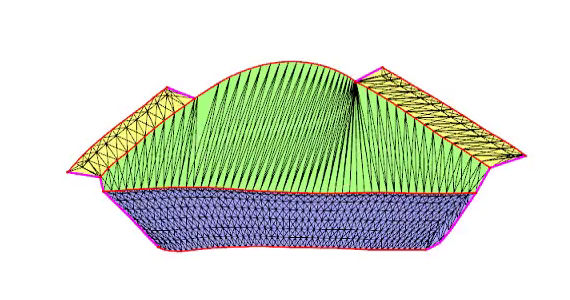
\includegraphics[width=.43\textwidth]{unErodeMesh1.png}&
	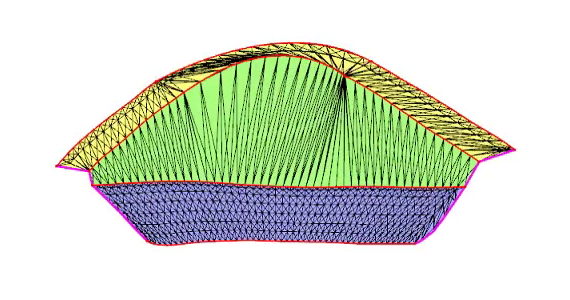
\includegraphics[width=.43\textwidth]{unErodeMesh2.png}\\
	\end{tabular}
	\caption{Un-Erode}
	\label{unerodecveg}
	\end{figure}
	\end{column}
	\begin{column}{0.55\textwidth}
	\begin{figure}[H]
	\centering
	\begin{tabular}{@{}cc@{}}
	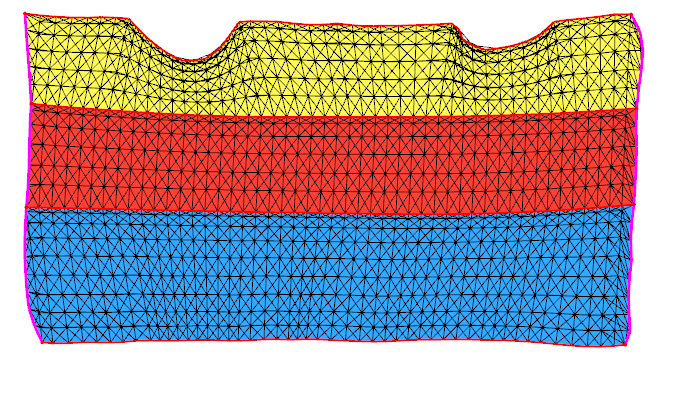
\includegraphics[width=.43\textwidth]{unErodehole0.png}&
	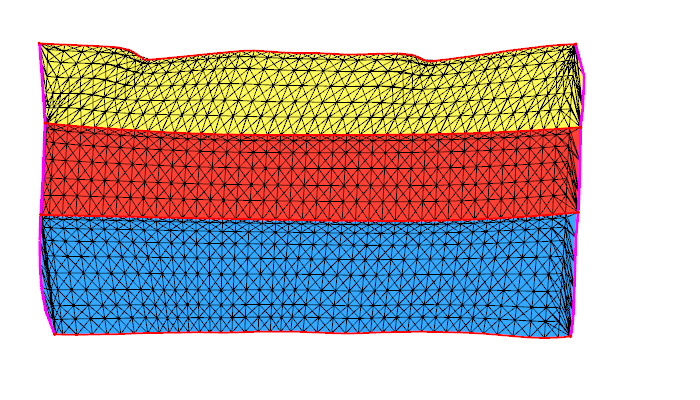
\includegraphics[width=.43\textwidth]{unErodehole1.png}\\
	\end{tabular}
	\caption{Un-Erode}
	\label{unfoldeg}
	\end{figure}
	\end{column}
	\end{columns}
	\end{frame}	
	
	\begin{frame}
	\frametitle{Event Simulation:  geological operators}
	\begin{figure}[H]
	\centering
	\href{un-fold.flv}{
\includegraphics[scale=0.2]{unFoldVid.png}}
	\caption{Un-Fold}
	\end{figure}
	\begin{figure}[H]
	\centering
	\href{un-Fault.flv}{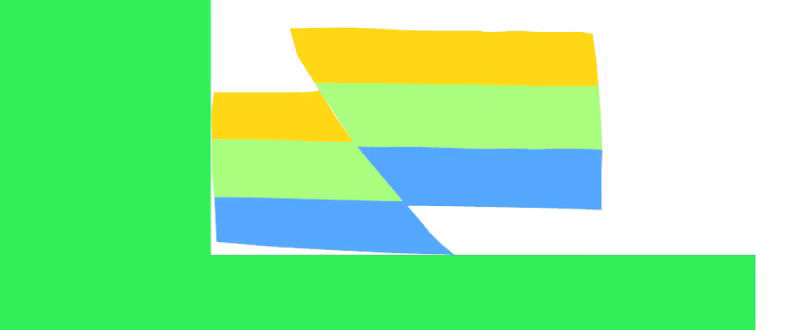
\includegraphics[scale=0.2]{unFaultVid.png}}
	\caption{Un-Fault}
	\end{figure}
	\end{frame}
	
	

	\begin{frame}
	\frametitle{Story Tree Generation}
	\begin{itemize}
	\item Recursion process: User choose events to un-do among a list a possible events to simulate $\longrightarrow$ simulation
	\item User can backtrack, continue or stop with the desired restoration
	\item System generate possible events list at step $t$: event with no time dependencies at time $t$ + dynamic events (un-erode for instance) + user events (un-fold).
	\item Process encoded into a Story Tree:
	\begin{itemize}
	\item Story Node $\longrightarrow$ possible events list
	\item Story Edge $\longrightarrow$ selected un-do events  list
	\end{itemize}

	\end{itemize}
	\end{frame}
	
	\begin{frame}
	\frametitle{Story Tree Generation}
	\begin{figure}[H]
	\centering
	\begin{tabular}{@{}cc@{}}
		\includegraphics[width=.35\textwidth]{ChartreuseDroiteEvent.png}&
	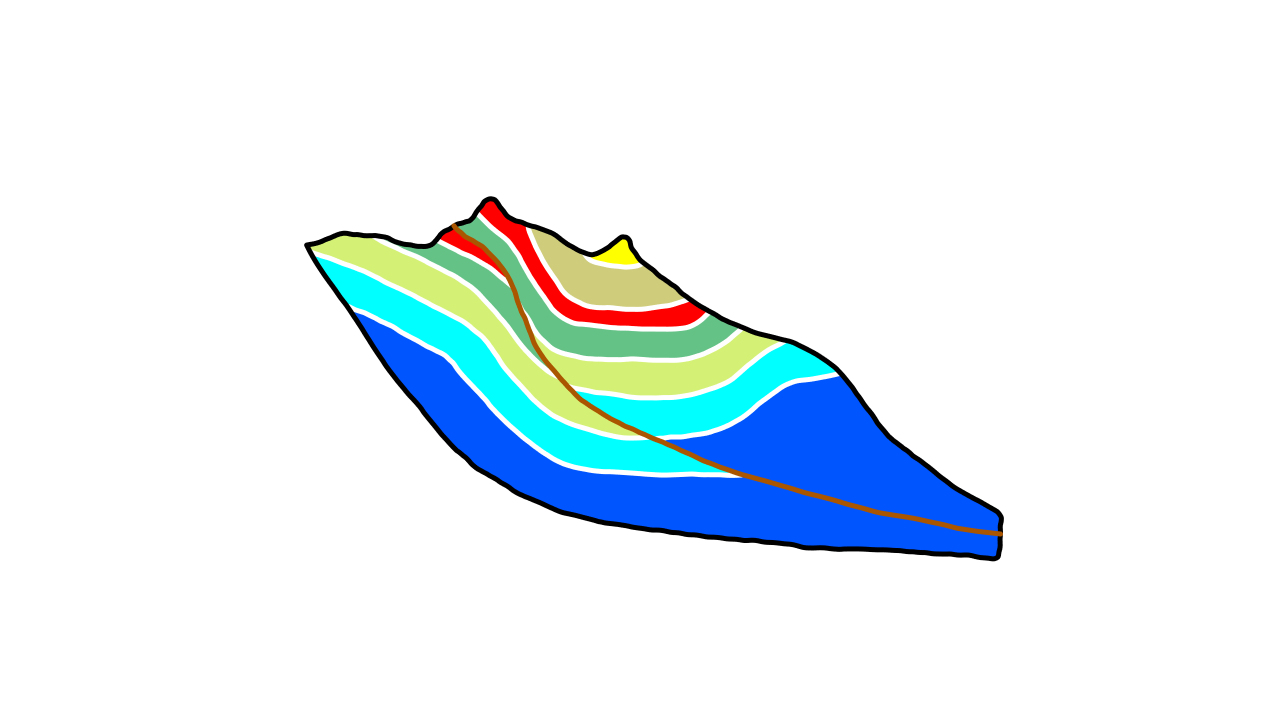
\includegraphics[width=.75\textwidth]{chartreusedroite.png}\\


	\end{tabular}
	\end{figure}
	\end{frame}
	
	\begin{frame}
	\frametitle{Restoration process}
	\begin{figure}[H]
	\centering
	\begin{tabular}{@{}cc@{}}
	\includegraphics[width=.35\textwidth]{RootNode.png}&
	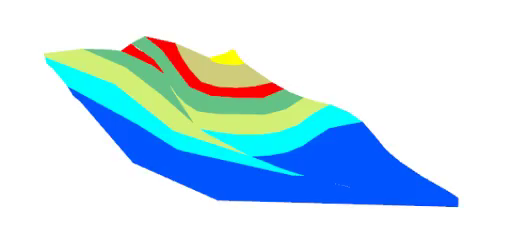
\includegraphics[width=.65\textwidth]{chartreusedroite0.png}\\
	\end{tabular}
	\end{figure}
	\end{frame}
	
	\begin{frame}
	\frametitle{Restoration process}
	\begin{figure}[H]
	\centering
	\begin{tabular}{@{}cc@{}}
	\includegraphics[width=.35\textwidth]{Node1a}&
	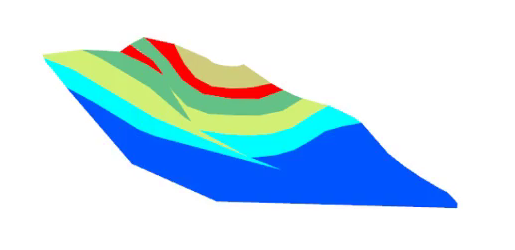
\includegraphics[width=.65\textwidth]{chartreusedroite1.png}\\
	\end{tabular}
	\end{figure}
	\end{frame}
	
	\begin{frame}
	\frametitle{Restoration process}
	\begin{figure}[H]
	\centering
	\begin{tabular}{@{}cc@{}}
	\includegraphics[width=.35\textwidth]{Node2a}&
	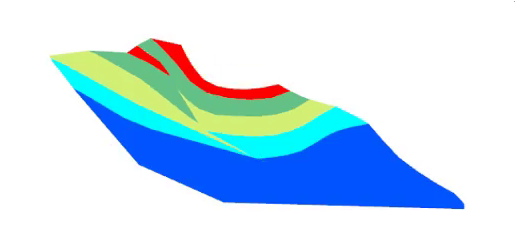
\includegraphics[width=.65\textwidth]{chartreusedroite2.png}\\
	\end{tabular}
	\end{figure}
	\end{frame}
	
	\begin{frame}
	\frametitle{Restoration process}
	\begin{figure}[H]
	\centering
	\begin{tabular}{@{}cc@{}}
	\includegraphics[width=.35\textwidth]{Node3a}&
	\includegraphics[width=.65\textwidth]{chartreusedroite5.png}\\
	\end{tabular}
	\end{figure}
	\end{frame}
	
	\begin{frame}
	\frametitle{Restoration process}
	\begin{figure}[H]
	\centering
	\begin{tabular}{@{}cc@{}}
	\includegraphics[width=.35\textwidth]{Node4a}&
	\includegraphics[width=.65\textwidth]{chartreusedroite6.png}\\
	\end{tabular}
	\end{figure}
	\end{frame}
	
	\begin{frame}
	\frametitle{Restoration process}
	\begin{figure}[H]
	\centering
	\begin{tabular}{@{}cc@{}}
	\includegraphics[width=.35\textwidth]{Node5a}&
	\includegraphics[width=.65\textwidth]{chartreusedroite7.png}\\
	\end{tabular}
	\end{figure}
	\end{frame}
	
	\begin{frame}
	\frametitle{Restoration process}
	\begin{figure}[H]
	\centering
	\begin{tabular}{@{}cc@{}}
	\includegraphics[width=.35\textwidth]{Node6a}&
	\includegraphics[width=.65\textwidth]{chartreusedroite8.png}\\
	\end{tabular}
	\end{figure}
	\end{frame}
		\begin{frame}
	\frametitle{Restoration process}
	\begin{figure}[H]
	\centering
	\begin{tabular}{@{}cc@{}}
	\includegraphics[width=.35\textwidth]{Node7a}&
	\includegraphics[width=.65\textwidth]{chartreusedroite9.png}\\
	\end{tabular}
	\end{figure}
	\end{frame}
	
	\begin{frame}
	\frametitle{Restoration process}
	\begin{figure}[H]
	\centering
	\begin{tabular}{@{}cc@{}}
	\includegraphics[width=.35\textwidth]{Node8a}&
	\includegraphics[width=.65\textwidth]{chartreusedroite10.png}\\
	\end{tabular}
	\end{figure}
	\end{frame}
	
	\begin{frame}
	\frametitle{Restoration process}
	\begin{figure}[H]
	\centering
	\begin{tabular}{@{}cc@{}}
	\includegraphics[width=.35\textwidth]{Node2b}&
	\includegraphics[width=.65\textwidth]{chartreusedroite25.png}\\
	\end{tabular}
	\end{figure}
	\end{frame}
	
	\begin{frame}
	\frametitle{Restoration process}
	\begin{figure}[H]
	\centering
	\begin{tabular}{@{}cc@{}}
	\includegraphics[width=.35\textwidth]{Node3b}&
	\includegraphics[width=.65\textwidth]{chartreusedroite26.png}\\
	\end{tabular}
	\end{figure}
	\end{frame}
	
	\begin{frame}
	\frametitle{Restoration process}
	\begin{figure}[H]
	\centering
	\begin{tabular}{@{}cc@{}}
	\includegraphics[width=.35\textwidth]{Node4b}&
	\includegraphics[width=.65\textwidth]{chartreusedroite27.png}\\
	\end{tabular}
	\end{figure}
	\end{frame}
	
	\begin{frame}
	\frametitle{Restoration process}
	\begin{figure}[H]
	\centering
	\begin{tabular}{@{}cc@{}}
	\includegraphics[width=.35\textwidth]{Node5b}&
	\includegraphics[width=.65\textwidth]{chartreusedroite28.png}\\
	\end{tabular}
	\end{figure}
	\end{frame}
	
	\begin{frame}
	\frametitle{Restoration process}
	\begin{figure}[H]
	\centering
	\begin{tabular}{@{}cc@{}}
	\includegraphics[width=.35\textwidth]{Node6b}&
	\includegraphics[width=.65\textwidth]{chartreusedroite29.png}\\
	\end{tabular}
	\end{figure}
	\end{frame}
		\begin{frame}
	\frametitle{Restoration process}
	\begin{figure}[H]
	\centering
	\begin{tabular}{@{}cc@{}}
	\includegraphics[width=.35\textwidth]{Node7b}&
	\includegraphics[width=.65\textwidth]{chartreusedroite210.png}\\
	\end{tabular}
	\end{figure}
	\end{frame}
	
	\begin{frame}
	\frametitle{Restoration process}
	\begin{figure}[H]
	\centering
	\begin{tabular}{@{}cc@{}}
	\includegraphics[width=.35\textwidth]{Node8b}&
	\includegraphics[width=.65\textwidth]{chartreusedroite10.png}\\
	\end{tabular}
	\end{figure}
	\end{frame}

		\begin{frame}
	\frametitle{Restoration process}
	\begin{figure}[H]
	\centering
	\begin{tabular}{@{}cc@{}}
	\includegraphics[width=.35\textwidth]{Node1c}&
	\includegraphics[width=.65\textwidth]{chartreusedroite31.png}\\
	\end{tabular}
	\end{figure}
	\end{frame}
	
	\begin{frame}
	\frametitle{Restoration process}
	\begin{figure}[H]
	\centering
	\begin{tabular}{@{}cc@{}}
	\includegraphics[width=.35\textwidth]{Node2c}&
	\includegraphics[width=.65\textwidth]{chartreusedroite32.png}\\
	\end{tabular}
	\end{figure}
	\end{frame}
	
	\begin{frame}
	\frametitle{Restoration process}
	\begin{figure}[H]
	\centering
	\begin{tabular}{@{}cc@{}}
	\includegraphics[width=.35\textwidth]{Node3c}&
	\includegraphics[width=.65\textwidth]{chartreusedroite33.png}\\
	\end{tabular}
	\end{figure}
	\end{frame}
	
	\begin{frame}
	\frametitle{Restoration process}
	\begin{figure}[H]
	\centering
	\begin{tabular}{@{}cc@{}}
	\includegraphics[width=.35\textwidth]{Node4c}&
	\includegraphics[width=.65\textwidth]{chartreusedroite34.png}\\
	\end{tabular}
	\end{figure}
	\end{frame}
	
	\begin{frame}
	\frametitle{Restoration process}
	\begin{figure}[H]
	\centering
	\begin{tabular}{@{}cc@{}}
	\includegraphics[width=.35\textwidth]{Node5c}&
	\includegraphics[width=.65\textwidth]{chartreusedroite35.png}\\
	\end{tabular}
	\end{figure}
	\end{frame}
	
	\begin{frame}
	\frametitle{Restoration process}
	\begin{figure}[H]
	\centering
	\begin{tabular}{@{}cc@{}}
	\includegraphics[width=.35\textwidth]{Node6c}&
	\includegraphics[width=.65\textwidth]{chartreusedroite37.png}\\
	\end{tabular}
	\end{figure}
	\end{frame}
		\begin{frame}
	\frametitle{Restoration process}
	\begin{figure}[H]
	\centering
	\begin{tabular}{@{}cc@{}}
	\includegraphics[width=.35\textwidth]{Node7c}&
	\includegraphics[width=.65\textwidth]{chartreusedroite38.png}\\
	\end{tabular}
	\end{figure}
	\end{frame}
	
	\begin{frame}
	\frametitle{Restoration process}
	\begin{figure}[H]
	\centering
	\begin{tabular}{@{}cc@{}}
	\includegraphics[width=.35\textwidth]{Node8c}&
	\includegraphics[width=.65\textwidth]{chartreusedroite10.png}\\
	\end{tabular}
	\end{figure}
	\end{frame}	
	

	\begin{frame}
	\frametitle{Experimental Results}
	%chartreuse bac? %more unit test?
	\begin{itemize}
	\item Restoration of Chartreuse cross-section
	\item Validation done by geologists 
	\end{itemize}
	\begin{figure}[H]
	\centering
	\href{chartreuseDroite-rev.mp4}
{\includegraphics[width=.65\textwidth]{chartreusedroite0.png}}
	\end{figure}
	\end{frame}
	
	\begin{frame}
	\frametitle{Limitation}
	%chartreuse bac? %more unit test?
	\begin{itemize}
	\item More validation should be done. Use more complex example like Chartreuse.
	\item Improve event operators to force layer thickness conservation 
	\item Mass-spring systems might not be the most suitable animation system for our context $\longrightarrow$ use more geometrical algorithm
	\end{itemize}
	\end{frame}
	
	\begin{frame}
	\frametitle{Future work}
	\begin{itemize}
	\item Take into account more geological events such as compaction or completly eroded materials
	\item Extend our space dimension to 3D $\longrightarrow$ take into account events such as Strike-slip faults
	\item Use and extend this storytelling process in other fields where storyboards are used (video games, cartoons)
	\end{itemize}
	\end{frame}
	
	\begin{frame}
	\frametitle{Conclusion}
	%chartreuse bac? %more unit test?
	\begin{itemize}
	\item New Storytelling based method for cross section restoration
	\item Use two graphs, Event (ranking) and Story (proposing) graph, for the storytelling process
	\item Proposed animation model using mass-springs systems. Created geological event simulation operators
	\item Proof of concept has been validated by geologists (Chartreuse and unit tests) and should be explored further.
	\end{itemize}
	\end{frame}
	

	
\end{document}